\chapter{Single-Agent Reinforcement Learning}
\label{chap:Reinforcement Learning}
\vspace{1cm}

In this chapter we introduce a reward-driven trial-and-error learning method, which is called \textit{reinforcement learning}, with a single agent in particular, and illustrate how to apply reinforcement learning to CO problems on graphs.

To describe the general idea of reinforcement learning, let us first consider a delivery truck shipping products from city \texttt{A} to city \texttt{B}, displayed as in \autoref{fig:delivery truck}. We assume that there are three different routes (route \texttt{a}, route \texttt{b}, route \texttt{c}) between those two cities, and they have different transportation cost, as in \autoref{fig:delivery truck}. To find the least-cost path, the delivery truck tries every route, records how much it costs the truck, and compare them. Here, the negative of transportation cost can be thought of as a reward. Eventually, the delivery truck learns that the route \texttt{c} produces the largest reward, and thus, it will always use the route \texttt{c} afterwards.
\begin{figure}[hbt!]
    \centering
    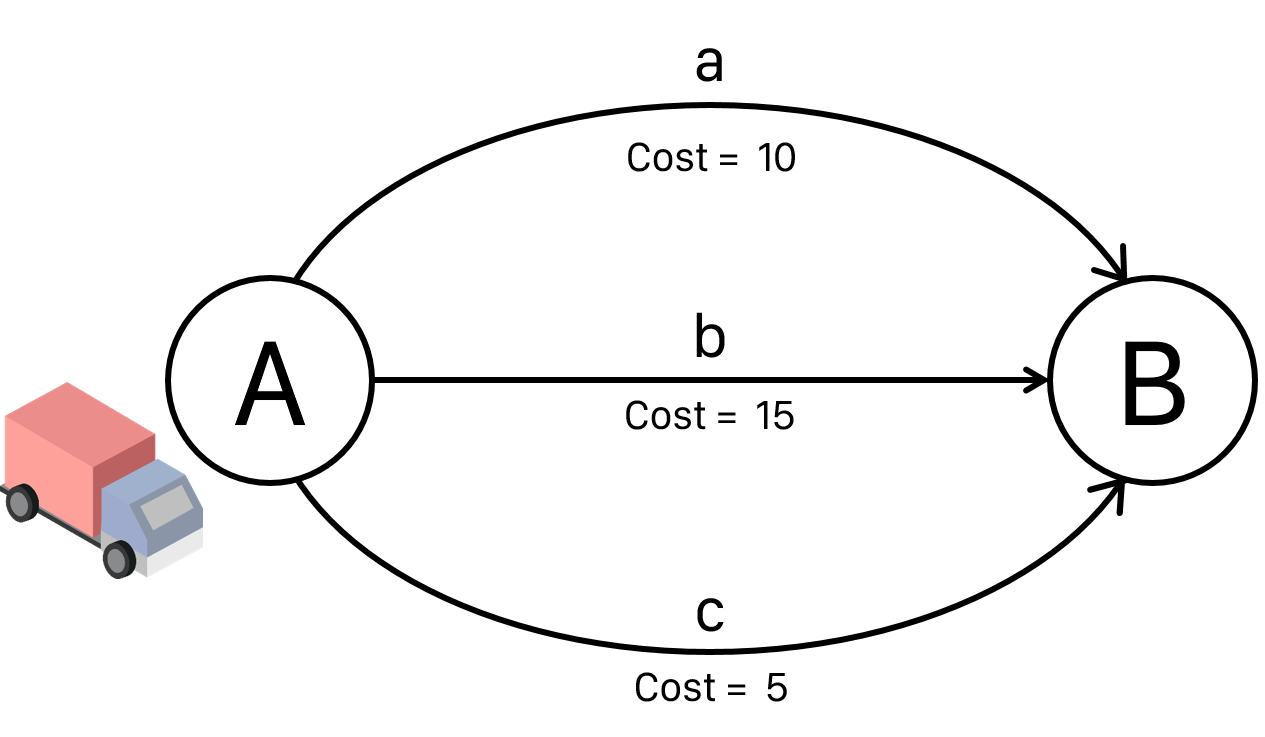
\includegraphics[width=0.65\textwidth]{figures/Reinforcement/truck.png}
    \captionsetup{justification=centering}
    \caption{Delivery truck example}
    \label{fig:delivery truck}
\end{figure}

The idea behind reinforcement learning is that its learning mechanism is driven by rewards from the environment a learning agent is interacting with. In order to maximize the reward, the agent learns what is the best decision to make from its experience of receiving a reward from the environment.

In our delivery truck example, the truck takes an action, which is to choose a specific route, and receives a corresponding reward -- the negative of transportation cost. The environment here can be considered as a function of a current city and action that returns a reward and the next city. For instance, if the delivery truck takes an action to select the route \texttt{a} from the city \texttt{A}, then the environment returns the city \texttt{B} and the reward -10. At the end, the delivery truck learns that choosing the route \texttt{c} is the best action to maximize the reward.

Reinforcement learning can be characterized by three noteworthy features. First of all, a learning agent has no instructor who directs which actions to choose, and thus, should try various actions until it discovers the best one that provides the biggest reward. Second, the main objective of reinforcement learning is to maximize the total amount of reward received from the environment, rather than investigate the hidden structure of unlabeled data. Finally, the agent has to \textit{exploit} the past experience to select the best action that offers the greatest reward, but also to \textit{explore} undiscovered actions for better rewards in the long run. To maximize a reward, a learning agent prefers to select actions that have yielded the most rewards from what has already been executed so far. The agent, however, has also to try other actions that have not been chosen in the past, since one of them may produce the biggest reward among all actions.

In our delivery truck example, no one tells which route should be taken, and thus, the truck explores all three routes to discover the least-cost route. Moreover, The delivery truck does not look into the transportation cost mechanism, but merely tries to maximize its reward. To describe the last key feature of reinforcement learning from the delivery truck example, let us assume that the truck has only tried the route \texttt{a} and route \texttt{b} at this moment. If the truck does not go further in its exploration of finding the best route and only exploits its past experience, then it will end up with choosing the route \texttt{a} as the best route, which is not true. Since it is impossible to perform both exploitation and exploration with a single action, the agent should balance them during the learning process to achieve the greatest reward at the end.

The first section of this chapter describes a \textit{Markov Decision Process} (MDP), which is a mathematical framework for designing problems where reinforcement learning methods with a single agent can be applied, and illustrates how a single-pair shortest path problem fit into this framework. In \autoref{sec: Tabular Solution Method}, we introduce a temporal-difference learning method, which is one of reinforcement learning methods for solving finite Markov decision problems. In particular, we look more closely at its off-policy case, which is known as Q-learning (\citeauthor{watkins1989learning} \cite{watkins1989learning}), and solve our single-pair shortest path problem using Q-learning. In \autoref{sec: value function approximation}, we extend the temporal-difference learning method with function approximation so that it can handle problems whose state space is significantly large. In \autoref{}


\section{Markov Decision Processes}
\label{sec: Markov Decision Process}
In this section, we present how to formulate reinforcement learning problems of maximizing cumulative reward with a single agent using the framework of Markov decision processes (MDPs), which comes from the field of optimal control. In reinforcement learning, much attention is given to cases where we approximate an optimal solution that is hard to find, and the exact model of problem is unknown. For more detailed discussion of historical influences of MDPs on reinforcement learning, see Chapter 1 and 3 of \citeauthor{sutton2018reinforcement} \cite{sutton2018reinforcement}.

Moreover, we consider a toy example of single-pair shortest path problem with an undirected graph, presented as in \autoref{fig:toy graph}, where it aims to find a path between origin node to destination node such that the sum of the transportation cost of its consisting edges is minimized.

\begin{figure}[hbt!]
    \centering
    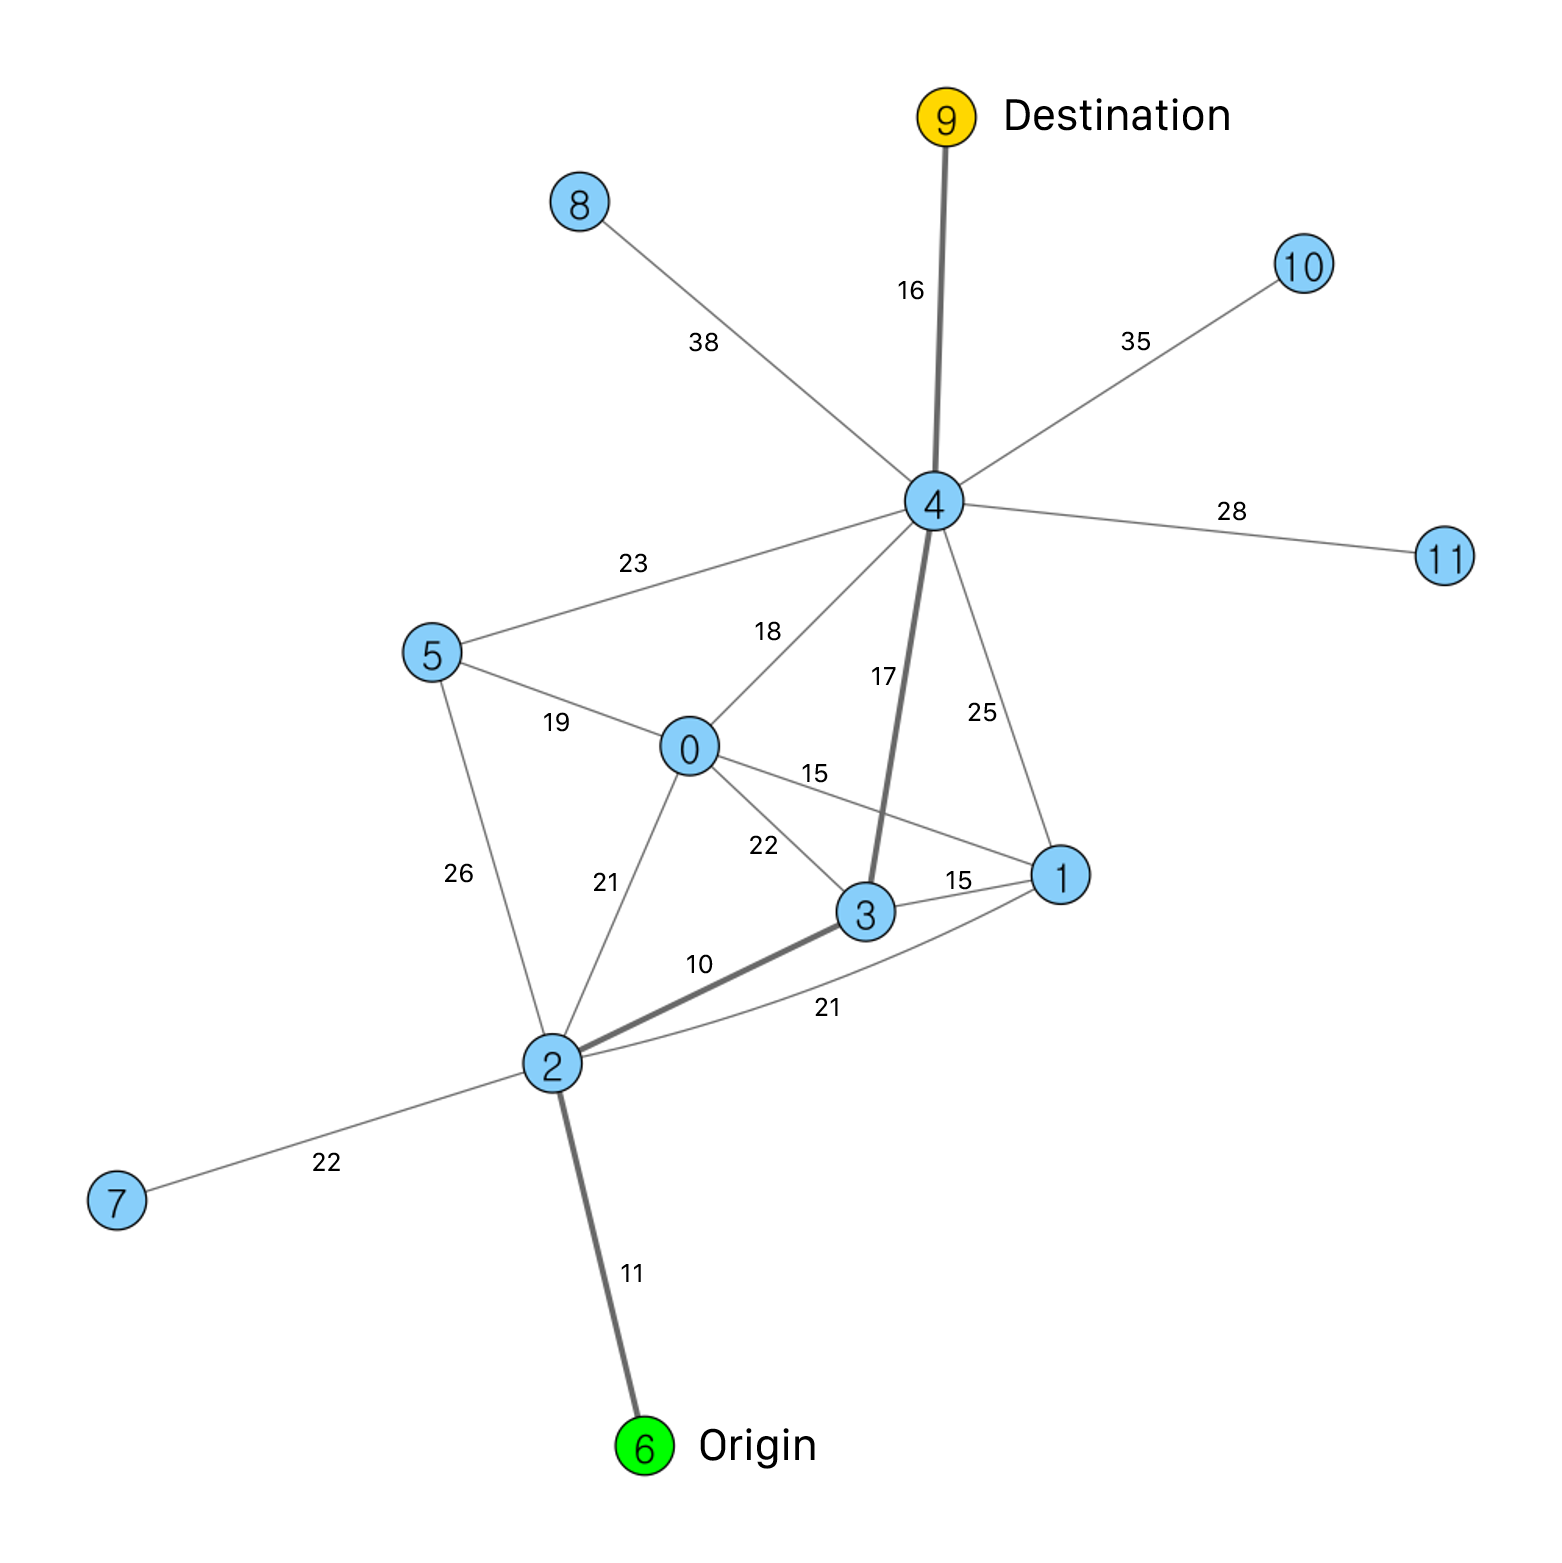
\includegraphics[width=0.95\textwidth]{figures/Reinforcement/figure1.png}
    \caption{\textbf{Example 1}: the shortest path is represented by the bold line. The number next to the edge is its transportation cost.}
    \label{fig:toy graph}
\end{figure}
\clearpage
\subsection{The Agent-Environment Interface}
The one who learns and makes a decision is called the \textit{agent}, and the world where the agent moves around is composed of three elements: set of all states, $\mathcal{S}$, set of all actions available in state $s \in \mathcal{S}$, denoted by $\mathcal{A}(s) \subset \mathcal{A}$, and set of all possible rewards, which is a subset of real number set, $\mathcal{R} \subset \mathbb{R}$.

\begin{figure}[hbt!]
    \centering
    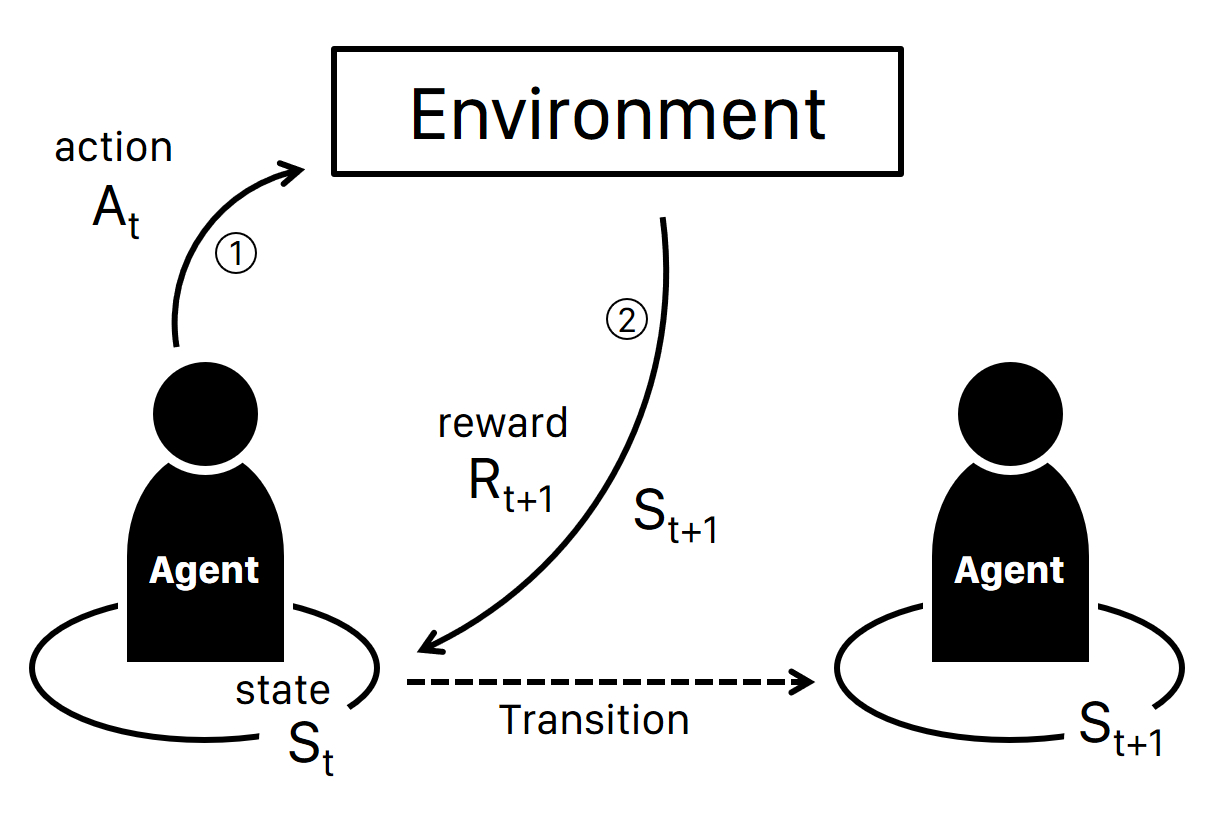
\includegraphics[width=0.7\textwidth]{figures/Reinforcement/interaction.pdf}
    \captionsetup{justification=centering}
    \caption{Agent-environment interaction}
    \label{fig:interaction}
\end{figure}

The system that the agent interacts with is called the \textit{environment}. To describe this more specifically, let us assume that the agent interacts with the environment at each of a sequence of discrete time steps, $t = 0,1,2, \dots$. At each time step $t$, the agent is given at a state $S_t \in \mathcal{S}$, and selects an action $A_t \in \mathcal{A}(S_t) \subset \mathcal{A}$, which is available in a given state $S_t$, and then two pieces of information, $(S_t, A_t)$, are transmitted to the environment. In the next time step, the environment grants the agent a reward $R_{t+1} \in \mathcal{R}$ and a new state, $S_{t+1}$. The process of agent-environment interaction is displayed in \autoref{fig:interaction}. A \textit{trajectory} that arises from such interaction can be illustrated by a sequence as follows:
\begin{align}S_0, A_0, R_1, S_1, A_1, R_2, S_2, A_2, R_3, S_3, \dots\end{align}
If states, actions, and rewards in MDP are discrete random variables with finite support, then it is called a \textit{finite} MDP. Let us now define \textit{state-reward-transition} probability function $p : \mathcal{S}\times\mathcal{R}\times\mathcal{S}\times\mathcal{A}\rightarrow[0,1]$ as follows:
\begin{align}
\label{eq:dynamics function}
p(s',r|s,a) := \text{Pr}\{S_t=s', R_t=r \ | \ S_{t-1} = s, A_{t-1} = a\},
\end{align}
for all $s',s\in \mathcal{S}, r\in\mathcal{R}$, and $a\in\mathcal{A}(s)$. The function $p$ provides a probability density function of $S_t$ and $R_t$, conditioning on the preceding state and action ($S_{t-1}$, $A_{t-1}$). This probability function $p$ defines the environment in reinforcement learning problems with a single agent.

Equation \eqref{eq:dynamics function} implies that the probability of each possible state and reward at a time step $t$ depends only on the value of $S_{t-1}$ and $A_{t-1}$, and thus, it is independent of all the states and actions that had happened before a time step $t-1$. Throughout this paper, we will assume that all the information about agent-environment interactions that occurred in the past must be reflected in the current state, which is then said to have the \textit{Markov property}.

From the four-argument state-reward-transition function $p$, one can derive a three-argument \textit{state-transition} probability function $\tilde{p}:\mathcal{S}\times\mathcal{S}\times\mathcal{A}\rightarrow[0,1]$ as follows:
\begin{align}
\label{eq:state-transition function}
\tilde{p}(s'|s,a) := \text{Pr}\{S_t=s' \ | \ S_{t-1} = s, A_{t-1} = a\} = \sum_{r\in\mathcal{R}}p(s',r|s,a)
\end{align}
In the following sections, we denote the state-transition function by $p(s'|s,a)$ with a slight abuse of notation for the convenience.

We can also define the expected rewards for state-action pairs as a two-argument function $r:\mathcal{S}\times\mathcal{A}\rightarrow\mathbb{R}$:
\begin{align}
\label{eq:reward function}
r(s,a) := \mathbb{E}[R_t|S_{t-1}=s, A_{t-1}=a]=\sum_{r\in\mathcal{R}}r\sum_{s'\in\mathcal{S}}p(s',r|s,a)
\end{align}

In \hyperref[fig:toy graph]{Example 1}, we have the following setup for a state $s$, set of all states $\mathcal{S}$, an action $a$, and set of all possible action in state $s$, $\mathcal{A}(s)$:

\begin{table}[!htbp]
\begin{tabular}{ccl}
    $\mathcal{S}$ & & $V = \{0,1,2, \dots, 11\}$  \\[0.5em]
    $s$ & & a node $i \in V$ \\[0.5em]
    $\mathcal{A}(s)$ & & $N(s) = \{j \in V \ | \ (s, j) \in E \}$\\[0.5em]
    $a$ & & choosing one of adjacent nodes $j \in N(s)$ of the current node $s$
\end{tabular}
\end{table}

\hyperref[fig:toy graph]{Example 1} uses a deterministic environment, meaning that the state-transition function and reward function are not stochastic but deterministic. Thus, the state-transition probability function in \hyperref[fig:toy graph]{Example 1} can be described as a deterministic rule $\tau(s,a): \mathcal{S} \times \mathcal{A}(s) \rightarrow \mathcal{S}$:
\begin{align}
    \tau(s,a) = a \quad \text{for all } s\in \mathcal{S} = V \text{ and } a \in \mathcal{A}(s) = N(s),
\end{align}
and we have the following reward function $r(s,a): \mathcal{S} \times \mathcal{A}(s) \rightarrow \mathbb{R}$:
\begin{align}
    r(s,a) = -c_{sa}  \quad \text{for all } s\in \mathcal{S} = V \text{ and } a \in \mathcal{A}(s) = N(s),
\end{align}
where $-c_{sa}$ is the negative of transportation cost on edge $(s,a)$.

\subsection{Returns and Episodes}
\label{subsec:returns and episodes}
In the beginning of this chapter, we have said that the learning agent aims to maximize the total amount of reward received from the environment. In this section we shall specify this with a formal expression. To begin with, we first introduce two types of reinforcement learning problems: \textit{episodic} task and \textit{continuing} task.

In episodic tasks, the whole learning process, which is comprised of numerous agent-environment interactions, can be divided into subsequences, which we call \textit{episodes}. Each episode spans from a \textit{starting state} $S_0$ to a \textit{terminal state} $S_T$ where $T$ is a final time step, and each episode begins independently of how the previous episode ends. 

\hyperref[fig:toy graph]{Example 1} is an episodic task with a starting state --- the origin node \texttt{6} --- and a terminal state --- the destination node \texttt{9}. Thus, the agent starts from the origin node \texttt{6}, and terminates the episode whenever it arrives at the destination node \texttt{9}.

When the learning problem is episodic, the agent chooses an action that maximizes the expected value of a \textit{return}, where the return is the sum of rewards. The return at a time step $t$, denoted by $G_t$, is defined as follows:
\begin{align}
    \label{eq:return-episodic}
    G_t := R_{t+1} + R_{t+2} + R_{t+3} + \cdots + R_{T},
\end{align}
where $T$ is a final time step.

In continuing tasks, on the other hand, the learning process becomes an on-going process without limit, rather than a collection of episodes. In this case, \eqref{eq:return-episodic} becomes an infinite sum with a final time step $T = \infty$, which could easily be infinite. Thus, we add a concept of discounting to \eqref{eq:return-episodic}, and therefore, in the continuing task we use a \textit{discounted return} $G_t$ at a time step $t$:
\begin{align}
\label{eq:return-continuing}
    G_t := R_{t+1} + \gamma R_{t+2} + \gamma^2 R_{t+3} + \cdots = \sum_{k=0}^{\infty}\gamma^k R_{t+k+1},
\end{align}
where $\gamma$ is a \textit{discount rate}, $0\leq \gamma \leq 1$. The discount rate determines the current worth of a future reward. As $\gamma$ approaches 1, future rewards are taken into consideration more significantly. If $\gamma < 1$ and the reward sequence $\{R_t\}$ is bounded, the infinite sum, \eqref{eq:return-continuing} is finite. In continuing case, the agent selects an action that maximizes the expected value of the discounted return at each time step.

We now establish the recursive relationship between the current return and the succeeding return, which is useful for theory of reinforcement learning:
\begin{align}
\label{eq: rewards recursive}
    G_t :=& R_{t+1} + \gamma R_{t+2} + \gamma^2 R_{t+3} + \gamma^3 R_{t+4} + \cdots \nonumber\\
    =& R_{t+1} + \gamma\left(R_{t+2} + \gamma R_{t+3} + \gamma^2 R_{t+4} + \cdots \right) \nonumber\\
    =& R_{t+1} + \gamma G_{t+1}
\end{align}

\subsubsection{Notational Remarks}
In the episodic task, we need to differentiate the set of all nonterminal states, denoted by $\mathcal{S}$, from the set of all states including the terminal states, denoted by $\mathcal{S}^+$. Thus, we slightly modify \eqref{eq:dynamics function} to be applied to episodic tasks as follows:
\begin{align}
    p(s',r|s,a) := \text{Pr}\{S_t=s', R_t=r \ | \ S_{t-1} = s, A_{t-1} = a\},
\end{align}
for all $s' \in \mathcal{S}^+, s \in \mathcal{S}, r \in \mathcal{R},$ and $a \in \mathcal{A}(s)$, where $p : \mathcal{S}^+ \times \mathcal{R} \times \mathcal{S} \times \mathcal{A} \rightarrow [0,1]$. \hyperref[fig:toy graph]{Example 1} then has $\mathcal{S} = V \setminus \{9\} \text{ and } \ \mathcal{S}^+ = V$.

Moreover, we shall use a single notation that can express both the episodic task and the continuing task for the sake of notational convenience. To this end, let us present two conventions that will be followed afterwards. First, we do not specify an episode number, since each episode is considered individually.

\hyperref[fig:toy graph]{Example 1}, for instance, its trajectory can be written as follows:
\begin{align*}
    \text{Episode 1 }&: S_0, A_0, R_1, S_1, A_1, R_2, S_2, A_2, R_3, S_3, \dots, S_{T-1}, A_{T-1}, R_{T}, S_{T}\\ 
    \text{Episode 2 }&: S_0, A_0, R_1, S_1, A_1, R_2, S_2, A_2, R_3, S_3, \dots, S_{T-1}, A_{T-1}, R_{T}, S_{T}\\
    \text{Episode 3 }&: S_0, A_0, R_1, S_1, A_1, R_2, S_2, A_2, R_3, S_3, \dots, S_{T-1}, A_{T-1}, R_{T}, S_{T}\\
    &\vdots\\
    \text{Episode I }&: S_0, A_0, R_1, S_1, A_1, R_2, S_2, A_2, R_3, S_3, \dots, S_{T-1}, A_{T-1}, R_{T}, S_{T},
\end{align*}
where $S_0 = 6$, $S_T = 9$, and I is the total number of episodes.

The other convention is that we define the return in the episodic as \eqref{eq:return-continuing}, and when the agent arrives at the terminal state, it will not transitioned to any other node and receive a reward of zero afterwards. Thus, in the episodic task, $S_t = S_T$ for $t = T+1, T+2, \dots$, and the return at a time step $t$ is formulated as in \eqref{eq:return-continuing} with $R_{T+1} = R_{T+2} = \dots = 0$ and $\gamma = 1$.

\subsection{Policies and Value Functions}
\label{subsection:policies and value functions}
During the learning process, the agent selects an action based on a \textit{policy}, $\pi(a|s)$, which maps from a given state $s$ to probabilities of choosing each action $a$ available at $s$:
\begin{align}
    \pi(a|s) := \text{Pr}(A_t=a|S_t=s),
\end{align}
for all $a\in\mathcal{A}(s)$ for each $s\in\mathcal{S}$.

We now consider two \textit{value functions}: \textit{state-value} function and \textit{action-value} function. Given a policy $\pi$, the former estimates the value of a given state in terms of the expected return, and the latter evaluates how good it is to execute a certain action in a given state with regard to the expected return. 

The \textit{state-value function for policy} $\pi$, denoted by $v_\pi(s)$, is defined as follows:
\begin{align}
    v_\pi(s) &:= \mathbb{E}_\pi[G_t \ | \ S_t=s] \nonumber \\
    &= \mathbb{E}_\pi\left[ \ \sum_{k=0}^{\infty}\gamma^kR_{t+k+1} \ | \ S_t=s \ \right], \text{ for all } s\in\mathcal{S}
\end{align}
In other words, $v_\pi(s)$ represents the expected return when the agent starts moving from a given state $s$ and keeps following the policy $\pi$ thereafter.
\clearpage
As in \eqref{eq: rewards recursive}, one can construct a recursive relationship between the value of a state $s$ and the value of its succeeding states $s'$ for any policy $\pi$ and any state $s$ in the following way:
\begin{align}
    v_\pi(s) :&= \mathbb{E}_\pi\left[G_t \ | \ S_t = s\right]\nonumber\\
    &= \mathbb{E}_\pi\left[R_{t+1} + \gamma G_{t+1} \ | \ S_t = s\right]\tag{by \autoref{eq: rewards recursive}} \nonumber\\
    &= \mathbb{E}_\pi\left[R_{t+1} \ | \ S_t = s\right] + \gamma\mathbb{E}_\pi\left[G_{t+1} \ | \ S_t=s \right]\tag{by linearity of expectation}\nonumber\\
    &= \sum_a\pi(a|s)\mathbb{E}_\pi\left[R_{t+1}|S_t=s, A_t=a\right]\nonumber\\
    &\quad + \gamma\sum_{s'}\text{Pr}\left(S_{t+1}=s'|S_t = s\right)\mathbb{E}_\pi\left[G_{t+1} \ | \ S_{t+1} = s', S_t = s\right]\tag{by law of total probability}\nonumber\\
    &=\sum_a\pi(a|s)\sum_r r\sum_{s'}p(s',r|s,a)\nonumber\\
    &\quad+\gamma\sum_a\pi(a|s)\sum_{s'}p\left(s'|s, a \right)\mathbb{E}_\pi\left[G_{t+1}|S_{t+1}=s', S_t=s\right]\tag{by \autoref{eq:reward function}} \nonumber\\
    &=\sum_a\pi(a|s)\sum_r r\sum_{s'}p(s',r|s,a)\nonumber\\
    &\quad+\gamma\sum_a\pi(a|s)\sum_{s'}\sum_{r}p\left(s',r|s,a\right)\mathbb{E}_\pi\left[G_{t+1}|S_{t+1}=s', S_t=s\right]\tag{by \autoref{eq:state-transition function}} \nonumber\\
    &=\sum_a\pi(a|s)\sum_r r\sum_{s'}p(s',r|s,a)\nonumber\\
    &\quad+\gamma\sum_a\pi(a|s)\sum_{s'}\sum_{r}p\left(s',r|s,a\right)\mathbb{E}_\pi\left[G_{t+1}|S_{t+1}=s'\right]\label{eq:bell-markov}\\
    &= \sum_a\pi(a|s)\sum_{s'}\sum_r p(s',r|s,a)\big[ r+\gamma\mathbb{E}_\pi\left[ G_{t+1} \ | \ S_{t+1}=s'\right]\big]\nonumber\\
    &=\sum_a\pi(a|s)\sum_{s',r} p(s',r|s,a)\big[ r+\gamma v_\pi(s')\big], \ \text{ for all }s\in\mathcal{S},\label{eq:Bellman Equation}
\end{align}
where $a\in\mathcal{A}(s), s' \in \mathcal{S}$, and $r\in\mathcal{R}$. We use the Markov property in \eqref{eq:bell-markov}. Equation \eqref{eq:Bellman Equation} is called the \textit{Bellman equation for }$v_\pi$, which implies that the value of a state $s$ must be equal to the sum of discounted value of the expected next state $s'$ and the corresponding expected reward.

In addition to the state-value function, one can define a value function of a state-action pair $(s,a)$, which is called \textit{action-value function for policy} $\pi$. The action-value function, denoted by $q_\pi(s,a)$, determines the value of taking an action $a$ in state $s$ under a policy $\pi$. Similarly to the state-value function, we define the action-value function as the expected return when the agent starts from a state $s$, executes an action $a$, and continues to follow a policy $\pi$ thereafter:
\begin{align}
    q_\pi(s,a) :&= \mathbb{E}_\pi[G_t \ | \ S_t=s, A_t=a] \nonumber\\
    &= \mathbb{E}_\pi\left[\sum_{k=0}^{\infty}\gamma^kR_{t+k+1} \ | \ S_t=s, A_t=a\right],
\end{align}
where $a\in \mathcal{A}(s)$ and $s\in\mathcal{S}$. As in \eqref{eq:Bellman Equation}, we can derive the relationship between the action-value function of the current state-action pair and the state-value function of the succeeding state as follows: 
\begin{align}
    q_\pi (s,a) =& \mathbb{E}_\pi \big[ R_{t+1} + \gamma G_{t+1} \ | \ S_t = s, A_t = a \big] \nonumber \\
    =& \mathbb{E}_\pi \big[ R_{t+1} \ | \ S_t = s, A_t = a \big] + \mathbb{E}_\pi \big[ \gamma G_{t+1} \ | \ S_t = s, A_t = a \big] \nonumber \\
    =& r(s,a) + \gamma \sum_{s'}p(s'|s,a)\mathbb{E}_\pi \big[ G_{t+1} \ | \ S_{t+1}=s', S_t=s, A_t = a \big]\nonumber\\
    =& \sum_r r \sum_{s'}p(s',r|s,a) + \gamma \sum_{s'}\sum_{r}p(s',r|s,a)\mathbb{E}_\pi\big[G_{t+1} \ | \ S_{t+1}=s' \big]\nonumber\\
    =& \sum_{s',r}p(s',r|s,a)\Big[ r + \gamma \mathbb{E}_\pi \big[G_{t+1} \ | \ S_{t+1}=s'\big]\Big]\nonumber\\
    =& \sum_{s',r}p(s',r|s,a)\big[ r + \gamma v_\pi(s')\big] \label{eq:reculsive-action-value}
\end{align}

\subsection{Optimal Policies and Optimal Value Functions}
To achieve the goal of reinforcement learning, which is to maximize the total amount of received rewards, we need to find an \textit{optimal policy} --- the one that is better than or equal to any other policies. Here, a policy $\pi$ is said to be better than a policy $\pi'$ if and only if $v_\pi(s) \geq v_{\pi'}(s)$ for all $s\in\mathcal{S}$. There may exist multiple optimal policies, and we denote all the optimal policy by $\pi_\ast$.

The state-value function that is shared among optimal policies is called the \textit{optimal state-value function}. The optimal stat-value function, denoted $v_*$, is then defined as:
\begin{align}
    v_*(s) := \max_\pi v_\pi(s), \qquad \text{for all } s\in\mathcal{S}.
\end{align}
We can also define the \textit{optimal action-value function}, denoted $q_*$, as follows:
\begin{align}
    q_*(s,a) := \max_\pi q_\pi(s,a),\qquad \text{for all } s\in\mathcal{S} \text{ and } a\in\mathcal{A}(s).
\end{align}
The relationship between the optimal action-value function $q_\ast$ and the optimal state-value function can be written as:
\begin{align}
    q_*(s,a) = \mathbb{E}[R_{t+1} + \gamma v_\ast(S_{t+1}) \ | \ S_t = s, A_t = a].
\end{align}

Let us now consider the Bellman equation for $v_\ast$, which is called \textit{Bellman optimality equation} for $\pi_\ast$:
\begin{align}
    v_\ast(s) :=& \max_{a\in\mathcal{A}(s)} q_{\pi_\ast}(s,a)\nonumber\\
    =& \max_a \mathbb{E}_{\pi_\ast}[G_t \ | \ S_t = s, A_t = a]\nonumber\\
    =& \max_a \mathbb{E}_{\pi_\ast}[R_{t+1} + \gamma G_{t+1} \ | \ S_t = s, A_t = a]\nonumber\\
    =& \max_a \mathbb{E}[R_{t+1} + \gamma v_\ast(S_{t+1}) \ | \ S_t = s, A_t = a]\\
    =& \max_a \sum_{s',r}p(s',r|s,a)[r+\gamma v_\ast(s')],\label{eq:Bellman optimality eq for v}
\end{align}
for all $s \in \mathcal{S}$.

The Bellman optimality equation for $q_\ast$ is then as follows:
\begin{align}
\label{eq:Bellman optimality q}
    q_\ast(s,a) =& \mathbb{E}\left[ R_{t+1} + \gamma \max_{a'}q_\ast(S_{t+1},a') \ | \ S_t = s, A_t = a \right]\nonumber\\
    =& \sum_{s',r}p(s',r|s,a)[r+\gamma \max_{a'}q_\ast(s',a')],
\end{align}
for all $s\in\mathcal{S}$ and $a\in\mathcal{A}(s)$.

Once we solve the Bellman optimality equations, the optimal policy can be derived easily. In case of solving \eqref{eq:Bellman optimality eq for v}, for each state $s$,
\begin{align*}
    \pi_\ast(a|s) > 0 \text{ if and only if } a = \underset{a'}{\text{argmax}}\sum_{s',r}p(s',r|s,a')[r+\gamma v_\ast(s')]
\end{align*}
When we have a solution of \eqref{eq:Bellman optimality q}, for any state s, we have:
\begin{align*}
    \pi_\ast(a|s) > 0 \text{ if and only if } a = \underset{a'}{\text{argmax}} \ q_\ast(s,a')
\end{align*}

Since the optimal policy is determined by either $v_\ast$ or $q_\ast$, solving Markov Decision Process, which is to find an optimal policy, can be reduced to solve the Bellman optimality equations. With this regard, one could say that a reinforcement learning method solves the Bellman optimality equations approximately, which will be presented in the following sections.

\section{Tabular Solution Method}
\label{sec: Tabular Solution Method}
In this section, we begin our study of solving finite Markov decision problems by considering a \textit{tabular method} where the approximate value functions can be displayed in the form of arrays, or tables. Since it uses a table to present the approximate value functions for every case, a tabular method is suitable for when the state and action space are not considerably large. When the state space is significantly large, however, we use a value function approximation, which is described in \autoref{sec: value function approximation}. While methods using the value function approximation only find approximate solutions, tabular methods can often provide exact solutions, meaning that the the optimal value function and the optimal policy can be found.

In \autoref{sec: Tabular Solution Method}, we focus mainly on one of the tabular solution methods, called \textit{temporal-difference} (TD) learning, which is more central and novel to reinforcement learning than any other tabular solution methods such as Dynamic Programming (DP) or Monte Carlo (MC) Methods (\citeauthor{sutton2018reinforcement} \cite{sutton2018reinforcement}). For more detailed description of DP and MC methods, the readers is referred to \citeauthor{sutton2018reinforcement} \cite{sutton2018reinforcement}. TD learning is a model-free method, meaning that the joint probability distribution of next-state ($S_{t+1}$) and reward ($R_{t+1}$) conditioning on the current state ($S_{t}$) and action ($A_{t}$) is not required. In other words, we do not need to specify the state-reward-transition function $p$ during the TD learning. Moreover, TD methods generally learn faster than MC methods. We shall look in more detail at the TD learning method in the following subsections.

The general idea of solving finite Markov decision problems is twofold: estimating the value function for a given policy, which is called \textit{policy evaluation} or \textit{prediction} problem, and finding an optimal policy, which is referred to as a \textit{control} problem. In \autoref{TD learning} we first consider TD prediction problem where we learn the state-value function $v_\pi$ for a given policy $\pi$. In \autoref{subsec: Q-learning} we move on to the control problem where we want to approximate optimal policies. In particular, we consider the off-policy case of TD control, which is called Q-learning (\citeauthor{watkins1989learning} \cite{watkins1989learning}), and apply this method to \hyperref[fig:toy graph]{Example 1}.

\subsection{Temporal-Difference Prediction}
\label{TD learning}
Suppose that we are given a policy $\pi$, and wish to estimate the state-value function $v_\pi$. In the simplest TD method, its estimate $V$ of $v_\pi$ is updated at each time step as follows:
\begin{align}
\label{TD prediction update rule}
    V(S_t) \leftarrow V(S_t) + \alpha \big[ R_{t+1} + \gamma V(S_{t+1}) - V(S_t) \big],
\end{align}
where $\alpha \in (0,1]$ is a learning rate. This update rule follows a general form of:
\begin{align}
\label{update_rule}
    \text{New Estimate} \leftarrow \text{Old Estimate} + \text{Step Size } \big[ \underbrace{\text{Target} - \text{Old Estimate}}_\text{Error}\big]
\end{align}
This form implies that the ``Old Estimate'' is desired to move in direction of the ``Target''.  In \eqref{TD prediction update rule} $R_{t+1} + \gamma V(S_{t+1})$ is the target and $V(S_t)$ is the old estimate. Recall from \autoref{subsection:policies and value functions} that
\begin{align}
    v_\pi(s) :&= \mathbb{E}_\pi\left[G_t \ | \ S_t = s\right]\nonumber\\
    &= \mathbb{E}_\pi\left[R_{t+1} + \gamma G_{t+1} \ | \ S_t = s\right] \nonumber\\
    &= \mathbb{E}_\pi\left[R_{t+1} + \gamma v_\pi(S_{t+1}) \ | \ S_t = s\right] \label{TD target}
\end{align}
As the expected value in \eqref{TD target} is not known in the TD learning method, the TD target, $R_{t+1} + \gamma V(S_{t+1})$, uses a sample value instead of the real expected values in \eqref{TD target}. Moreover, the current estimate V replaces the true $v_\pi$ in \eqref{TD prediction update rule}. \citeauthor{sutton1988learning} \cite{sutton1988learning} proves that the expected value of estimate V in \eqref{TD prediction update rule} converges to the true $v_\pi$, and \citeauthor{dayan1992convergence} \cite{dayan1992convergence} shows the proof of convergence with probability 1.

The ``error'' term in \eqref{TD prediction update rule}, $R_{t+1} + \gamma V(S_{t+1}) - V(S_t)$, is called the \textit{TD error} defined as:
\begin{align}
    \delta_t := R_{t+1} + \gamma V(S_{t+1}) - V(S_t).
\end{align}
Since the target $R_{t+1} + \gamma V(S_{t+1})$ depends on the next state and next reward, the TD error $\delta_t$ can be seen as a temporal error, meaning that this error is valid only at time $t+1$. The name TD stems from its use of temporal difference between successive estimates of the value function.

The following algorithm shows how to estimate $v_\pi$ given a policy $\pi$ using the TD method.

\begin{algorithm}[H]
\SetAlgoLined
 Algorithm parameters: step size $\alpha \in (0,1]$ \\
 \text{Initialize } $V(s), \text{ for all } s\in \mathcal{S}^+$ \\
 \For{each episode}{
  Initialize $S$\\
  \While{$S$ is not a terminal state}{
   Choose $A$ from $S$ using the given policy $\pi$\\
   Execute $A$, observe $R, S'$\\
   $V(S) \leftarrow V(S) + \alpha\big[ R + \gamma V(S') - V(S)\big]$\\
   $S \leftarrow S'$
   }
 }
 \caption{Tabular TD for estimating $v_\pi$ given a policy $\pi$}
\end{algorithm}

\subsection{Q-learning: Off-policy TD Control}
\label{subsec: Q-learning}
We now consider the control problem where we wish to find an optimal policy using TD prediction methods. Suppose that we want to find a new greedy policy, $\pi'$ given the state-value function for the current policy $\pi$, $v_\pi(s)$, for $\forall s\in \mathcal{S}$. Then we have:
\begin{align}
    \pi'(s) :=& \ \underset{a}{\text{argmax}} \ q_\pi(s,a)\nonumber\\
    =& \ \underset{a}{\text{argmax}}  \ \mathbb{E}\big[R_{t+1} + \gamma v_\pi(S_{t+1}) \ | \ S_t = s, A_t = a\big]\nonumber\\
    =& \ \underset{a}{\text{argmax}} \sum_{s', r} p(s', r | s, a)\big[r + \gamma v_\pi(s')\big] \label{policy improvement}
\end{align}
From \eqref{policy improvement}, it can be clearly seen that the state values alone are not sufficient to determine a policy if a model is not available, meaning that the conditional probability distribution of the next state and reward is not known. Since TD learning has no information about a model, we now estimate the action-value function instead of the state-value function for the control problem.

Before we look more closely at the TD control problem, we want to describe two learning approaches to the control problem: \textit{on-policy learning} and \textit{off-policy learning}. In the beginning of this chapter, we have said that balancing between exploration and exploitation is important in reinforcement learning. Suppose that a learning agent exclusively selects an action that produces the most reward at the moment, which is called \textit{greedy action}. Then the agent may lose the opportunity to find a better action than the current greedy action unless it is an optimal action; thus, we need to maintain exploration to ensure the greater return in the long run. To assure that the agent selects all actions continually often, two approaches--on-policy learning and off-policy learning--have been introduced.

In on-policy methods, the agent evaluates or improves the policy that is also used for exploration. In off-policy methods, however, two different policies -- \textit{target policy} and \textit{behavior policy} -- are used for learning and exploration respectively. In other words, the agent uses the behavior policy to explore all possible actions, and learns only the target policy which converges to an optimal policy. One benefit of separating the target policy from the behavior policy is that we may obtain a deterministic optimal policy, while continuing to pursue exploration using a non-deterministic policy, such as an \textit{$\varepsilon$-greedy} policy where $\varepsilon \in (0,1)$ is an exploration rate. $\varepsilon$-greedy policy chooses a greedy action with probability $1-\varepsilon$, and performs an exploration with probability $\varepsilon$, where the action is selected uniformly at random. Off-policy methods often show greater variance and slower convergence compared to on-policy methods, since the target policy is learned with the data which is generated by the different policy, the behavior policy. Despite such limitation, off-policy approaches have attracted much attention of researchers due to its various application domains.
\clearpage

We now present an off-policy TD control algorithm, known as \textit{Q-learning} (\citeauthor{watkins1989learning} \cite{watkins1989learning}). Q-learning updates the estimate of action-value function, denoted by $Q$, as follows:

\begin{algorithm}[H]
\SetAlgoLined
 Algorithm parameters: step size $\alpha \in (0,1], \text{ small } \varepsilon > 0$ \\
 \text{Initialize } $Q(s,a), \text{ for all } s\in \mathcal{S}^+, a\in\mathcal{A}(s)$ \\
 \For{each episode}{
  Initialize $S$\\
  \While{$S$ is not a terminal state}{
   Choose $A$ from $S$ using policy derived from $Q$ (e.g., $\varepsilon$-greedy)\\
   Execute $A$, observe $R, S'$\\
   $Q(S,A) \leftarrow Q(S,A) + \alpha\big[ R + \gamma \max_a Q(S', a) - Q(S, A)\big]$\\
   $S \leftarrow S'$
   }
 }
 \caption{Q-learning}
\end{algorithm}
As in the 6th row of Q-learning algorithm, the agent explores all possible actions using the behavior policy, such as $\varepsilon$-greedy policy, derived from the action-value function estimates, $Q$. Moreover, $\max_a Q(S', a)$ is used as a target policy, as in the 8th row. Since two different policies are used, Q-learning is an off-policy method.

\subsection{Application of Q-learning to Example 1}
We have implemented Q-learning for \hyperref[fig:toy graph]{Example 1} with the following hyperparameters:
$$\alpha = 1, \gamma = 1, \varepsilon = 0.1.$$
The learning rate $\alpha$ determines how much the new samples  $(s,a,s',r)$ from the state-reward-transition function can affect our current action-value function estimates. In stochastic environment where its state-transition function has randomness, high learning rate may cause unstable learning, and thus low learning rate is commonly used. If the learning procedure is slow with low learning rate, a great deal of samples are used to update the estimates, so that we can stabilized the learning process. In deterministic environment, however, there is no randomness in transition functions, and thus, the learning stability is not affected by the learning rate. Hence, we set the learning rate $\alpha$ to one.

Moreover, the discount rate $\gamma$ is set to 1, meaning that the current reward is worth as much as the future rewards. Note that the reward in \hyperref[fig:toy graph]{Example 1} is defined as the negative of the transportation cost on the edge. As every single of the transportation costs charged in one episode is worth equally, we set the discount rate $\gamma$ to 1.

The performance of Q-learning method on \hyperref[fig:toy graph]{Example 1} is displayed in \autoref{fig:q-learning graph}. The approximated optimal policy and the action-value function estimates $Q(s,a)$ are illustrated in \autoref{tab:Q(s,a)}. The path derived from our learned action-value function Q turns out to be the same as the exact solution, which is presented in \autoref{fig:toy graph}.

To check if the action-value function estimates $Q(s,a)$ obtained after 50000 episodes satisfy the Bellman optimality equation, let us consider an state-action pair $(s,a) = (6,2)$, for instance. The following equations show that $Q(6,2)$ satisfies the Bellman optimality equation:

\begin{align*}
    -54 = Q(6,2) &= \sum_{s',r}p(s',r | 6,2)[r + 1\cdot \max_{a'} Q(s',a')]\\
    &= -11 + 1 \cdot \max_{a'} Q(2,a')\\
    &= -11 + 1 \cdot Q(2,3)\\
    &= -11 + 1 \cdot (-43)\\
    &= -54
\end{align*}

\begin{figure}[hbt!]
    \centering
    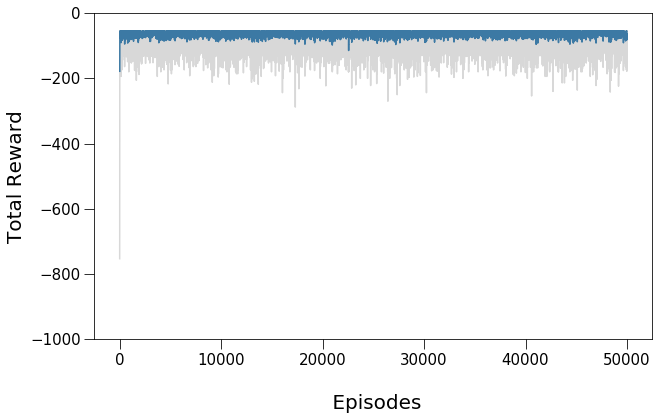
\includegraphics[width=0.9\textwidth]{figures/Reinforcement/performance.png}
    \caption{Performance of Q-learning method in \hyperref[fig:toy graph]{Example 1}. The grey line represents the sum of rewards during episode, and the blue line displays a moving average of 10 episodes.}
    \label{fig:q-learning graph}
\end{figure}

\begin{table}[!htbp]
\begin{adjustbox}{width=\columnwidth,center}
\begin{tabular}{@{\extracolsep{5pt}} cccccccccccccc} 
\\[10ex]\hline 
\hline \\[-1.8ex]
& \multicolumn{12}{c}{Action} & Target\\
State & 0 & 1 & 2 & 3 & 4 & 5 & 6 & 7 & 8 & 9 & 10 & 11 & Policy\\ 
\hline \\[-1.8ex] 
0 & $-$ & $-56$ & $-64$ & $-55$ & $-34$ & $-58$ & $-$ & $-$ & $-$ & $-$ & $-$ & $-$ & [4]\\ 
1 & $-49$ & $-$ & $-64$ & $-48$ & $-41$ & $-$ & $-$ & $-$ & $-$ & $-$ & $-$ & $-$ & [4] \\ 
2 & $-55$ & $-62$ & $-$ & $-43$ & $-$ & $-65$ & $-65$ & $-87$ & $-$ & $-$ & $-$ & $-$ & [3]\\ 
3 & $-56$ & $-56$ & $-53$ & $-$ & $-33$ & $-$ & $-$ & $-$ & $-$ & $-$ & $-$ & $-$ & [4]\\ 
4 & $-52$ & $-66$ & $-$ & $-50$ & $-$ & $-62$ & $$ & $$ & $-92$ & $-16$ & $-86$ & $-72$ & [9] \\ 
5 & $-53$ & $-$ & $-69$ & $-$ & $-39$ & $-$ & $-$ & $-$ & $-$ & $-$ & $-$ & $-$ & [4]\\ 
6 & $-$ & $-$ & $-54$ & $-$ & $-$ & $-$ & $-$ & $-$ & $-$ & $-$ & $-$ & $-$ & [2]\\ 
7 & $-$ & $-$ & $-65$ & $-$ & $-$ & $-$ & $-$ & $-$ & $-$ & $-$ & $-$ & $-$ & [2]\\ 
8 & $-$ & $-$ & $-$ & $-$ & $-54$ & $-$ & $-$ & $-$ & $-$ & $-$ & $-$ & $-$ & [4]\\ 
9& $-$ & $-$ & $-$ & $-$ & $0$ & $-$ & $-$ & $-$ & $-$ & $-$ & $-$ & $-$ &\\ 
10 & $-$ & $-$ & $-$ & $-$ & $-51$ & $-$ & $-$ & $-$ & $-$ & $-$ & $-$ & $-$ & [4]\\ 
11 & $-$ & $-$ & $-$ & $-$ & $-44$ & $-$ & $-$ & $-$ & $-$ & $-$ & $-$ & $-$ & [4]\\ 
\hline \\[5ex] 
\end{tabular}
\end{adjustbox}
  \caption{Table of action-value function estimates $Q(s,a)$ and the target policy after training 50000 episodes}
  \label{tab:Q(s,a)} 
\end{table} 
\clearpage
Let us now look more closely at how our Q-learning algorithm approximates the optimal policy. \autoref{fig:walk_length} and \autoref{fig:walk_length_50000} shows the length of agent's walk from the starting state to the terminal node in each episode, which is the same as the total time steps in one episode. \autoref{tab:the first episode} presents quadruple of events $(S_t, A_t, S_{t+1}, R_{t+1})$, updated $Q(S_t, A_t)$, and updated $\underset{a}{\text{argmax }} Q(S_t, a)$ at each time step in the first episode.

We can clearly see that it takes many time steps to arrive at the terminal state from the starting state at the beginning, since the agent does not have much information. As the agent goes through many episodes, however, it reaches the destination node much faster as illustrated in \autoref{fig:walk_length}.

Moreover, \autoref{fig:walk_length} and \autoref{fig:walk_length_50000} depict that the agent continues exploring with a behavior policy, which is an $\varepsilon$-greddy policy. Even though the agent is able to arrive at the terminal node with the minimum length, which is 4, roughly after 100th episode, the walk length is often greater than 4 during the whole training process.

\begin{figure}[hbt!]
    \centering
    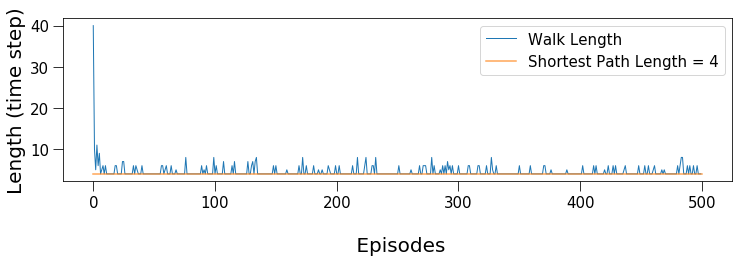
\includegraphics[width=0.9\textwidth]{figures/Reinforcement/walk_length_500.png}
    \caption{The length of agent's walk from the starting state (\texttt{node 6}) to the terminal state (\texttt{node 9}) in the first 500 episodes}
    \label{fig:walk_length}
\end{figure}
\begin{figure}[hbt!]
    \centering
    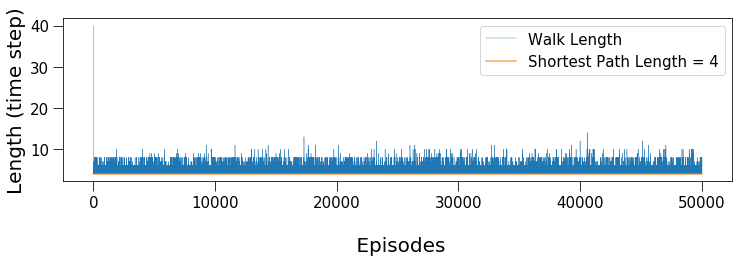
\includegraphics[width=0.9\textwidth]{figures/Reinforcement/walk_length.png}
    \caption{The length of agent's walk from the starting state (\texttt{node 6}) to the terminal state (\texttt{node 9}) during the whole training process}
    \label{fig:walk_length_50000}
\end{figure}

\begin{table}[!htbp]
\small
\begin{adjustbox}{totalheight = \textheight-4\baselineskip, center}
\begin{tabular}{@{\extracolsep{5pt}} ccccccc} 
\\[-1.8ex]\hline 
\hline \\[-1.8ex]
& State & Action & Next State & Reward & Updated & Updated \\
$t$ & $S_t$ & $A_t$ & $S_{t+1}$ & $R_{t+1}$ & $Q(S_t, A_t)$ & $\underset{a}{\text{argmax }} Q(S_t, a)$\\[1ex] 
\hline \\[-1.8ex] 
0 & 6 & 2 & 2 & -11 & -11 & [2] \\
1 & 2 & 0 & 0 & -21 & -21 & [1, 3, 5, 6, 7] \\
2 & 0 & 1 & 1 & -15 & -15 & [2, 3, 4, 5] \\
3 & 1 & 0 & 0 & -15 & -15 & [2, 3, 4] \\
4 & 0 & 2 & 2 & -21 & -21 & [3, 4, 5] \\
5 & 2 & 3 & 3 & -10 & -10 & [1, 5, 6, 7] \\
6 & 3 & 1 & 1 & -15 & -15 & [0, 2, 4] \\
7 & 1 & 2 & 2 & -21 & -21 & [3, 4] \\
8 & 2 & 1 & 1 & -21 & -21 & [5, 6, 7] \\
9 & 1 & 3 & 3 & -15 & -15 & [4] \\
10 & 3 & 2 & 2 & -10 & -10 & [0, 4] \\
11 & 2 & 5 & 5 & -26 & -26 & [6, 7] \\
12 & 5 & 4 & 4 & -23 & -23 & [0, 2] \\
13 & 4 & 0 & 0 & -18 & -18 & [1, 3, 5, 8, 9, 10, 11] \\
14 & 0 & 3 & 3 & -22 & -22 & [4, 5] \\
15 & 3 & 0 & 0 & -22 & -22 & [4] \\
16 & 0 & 4 & 4 & -18 & -18 & [5]  \\
17 & 4 & 1 & 1 & -25 & -25 & [3, 5, 8, 9, 10, 11] \\
18 & 1 & 4 & 4 & -25 & -25 & [0, 3]  \\
19 & 4 & 3 & 3 & -17 & -17 & [5, 8, 9, 10, 11] \\
20 & 3 & 4 & 4 & -17 & -17 & [2] \\
21 & 4 & 5 & 5 & -23 & -23 & [8, 9, 10, 11]  \\
22 & 5 & 0 & 0 & -19 & -19 & [2] \\
23 & 0 & 5 & 5 & -19 & -19 & [1] \\
24 & 5 & 2 & 2 & -26 & -26 & [0] \\
25 & 2 & 6 & 6 & -11 & -22 & [7] \\
26 & 6 & 2 & 2 & -11 & -11 & [2] \\
27 & 2 & 7 & 7 & -22 & -22 & [3] \\
28 & 7 & 2 & 2 & -22 & -32 & [2]  \\
29 & 2 & 3 & 3 & -10 & -20 & [3]  \\
30 & 3 & 2 & 2 & -10 & -30 & [1] \\
31 & 2 & 3 & 3 & -10 & -25 & [0, 1]  \\
32 & 3 & 1 & 1 & -15 & -30 & [4] \\
33 & 1 & 0 & 0 & -15 & -30 & [3] \\
34 & 0 & 1 & 1 & -15 & -30 & [4]  \\
35 & 1 & 3 & 3 & -15 & -32 & [2] \\
36 & 3 & 4 & 4 & -17 & -17 & [4] \\
37 & 4 & 8 & 8 & -38 & -38 & [9, 10, 11]  \\
38 & 8 & 4 & 4 & -38 & -38 & [4] \\
39 & 4 & 9 & 9 & -16 & -16 & [10, 11]  \\
\hline \\[-1.8ex] 
\end{tabular}
\end{adjustbox}
  \caption{Quadruple of events $(S_t, A_t, S_{t+1}, R_{t+1})$, updated $Q(S_t, A_t)$, and the target policy in the first episode of the training}
  \label{tab:the first episode} 
\end{table} 

The following four graphs demonstrate how the action-value function estimates converges in state 1,2,3, and 4 with two different learning rate $\alpha = 0.1, \alpha = 1.0$. It can clearly seen that the learning speed is faster in case of $\alpha=1.0$ and the learning is stable even with a high learning rate $\alpha = 1.0$ due to the deterministic environment.

In each state, the action-value estimate of the optimal action firstly converges to the optimal value among those of all possible actions, since the target term with an optimal action in the Q-learning update, $R + \gamma \max_a Q(S', a)$ as in the 8th row in the Algorithm 2, becomes stable first. For example, in state 4 with an action to choose \texttt{node 9} --- the optimal action in state 4 --- we have:
\begin{align*}
    R + \gamma \max_a Q(S', a) &= -16 + 1 \cdot \max_a Q(9, a)\\
    &= -16 + 1 \cdot 0\\
    &= -16
\end{align*}
The target term for $Q(4,9)$ in the Q-learning update rule is always -16 from the beginning, and thus, the action-value estimate $Q(4,9)$ converges first to the optimal value among all estimates, as in \autoref{fig:Q4 convergence}. The value of target term for all possible action in state 4 is presented in \autoref{fig:Q4 target}.

\begin{figure}[hbt!]
    \centering
    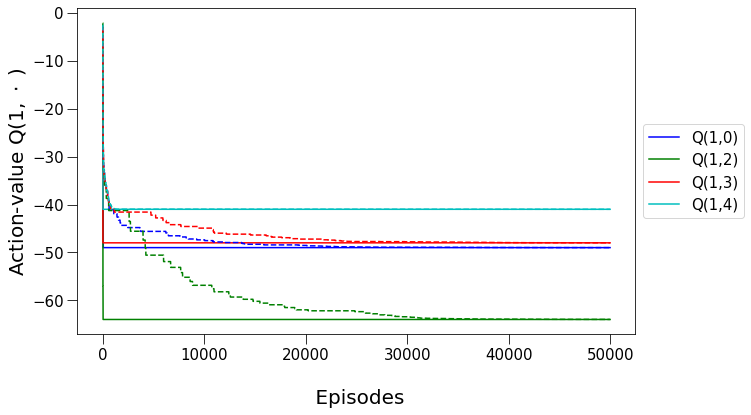
\includegraphics[width=0.9\textwidth]{figures/Reinforcement/Q1.png}
    \caption{Action-value function estimates Q for all possible action in state 1 with $\alpha = 1.0$ (solid line), and $\alpha = 0.1$ (dashed line)}
    \label{fig:Q1 convergence}
\end{figure}

\begin{figure}[hbt!]
    \centering
    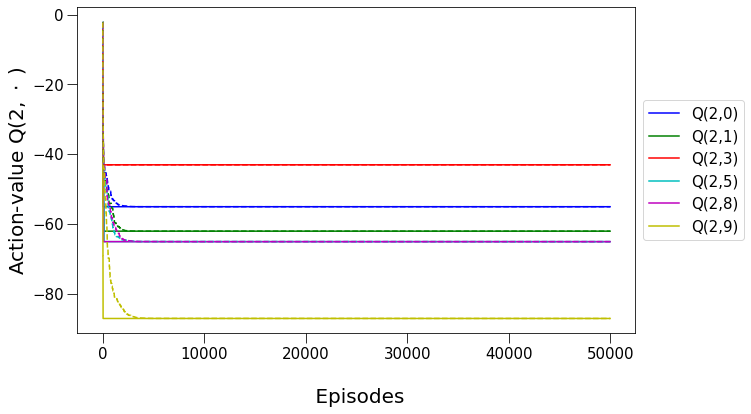
\includegraphics[width=0.9\textwidth]{figures/Reinforcement/Q2.png}
    \caption{Action-value function estimates Q for all possible action in state 2 with $\alpha = 1.0$ (solid line), and $\alpha = 0.1$ (dashed line)}
    \label{fig:Q2 convergence}
\end{figure}

\begin{figure}[hbt!]
    \centering
    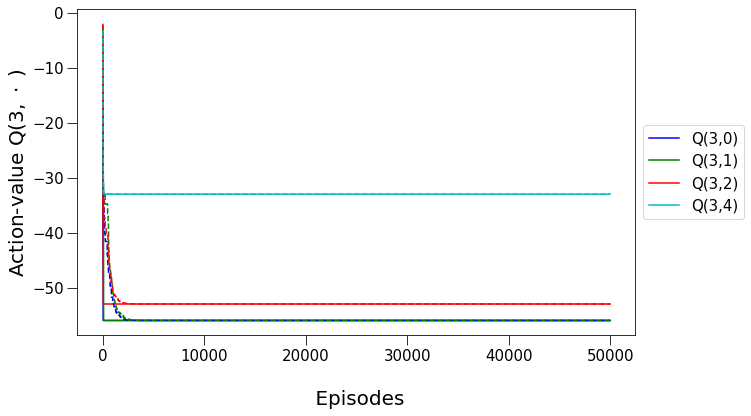
\includegraphics[width=0.9\textwidth]{figures/Reinforcement/Q3.png}
    \caption{Action-value function estimates Q for all possible action in state 3 with $\alpha = 1.0$ (solid line), and $\alpha = 0.1$ (dashed line)}
    \label{fig:Q3 convergence}
\end{figure}

\begin{figure}[hbt!]
    \centering
    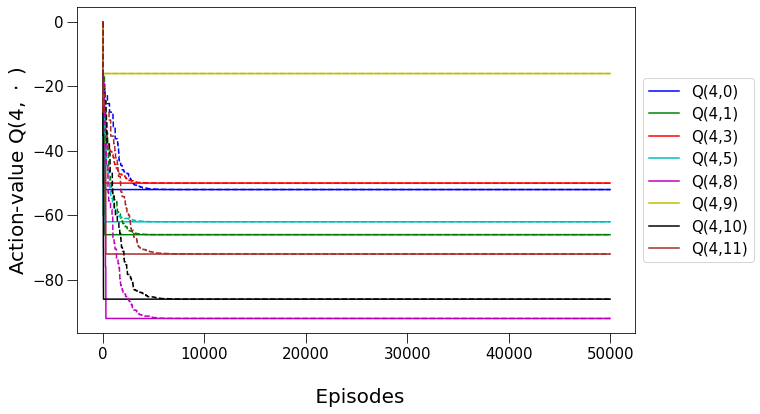
\includegraphics[width=0.9\textwidth]{figures/Reinforcement/Q4.png}
    \caption{Action-value function estimates Q for all possible action in state 4 with $\alpha = 1.0$ (solid line), and $\alpha = 0.1$ (dashed line)}
    \label{fig:Q4 convergence}
\end{figure}

\begin{figure}[hbt!]
    \centering
    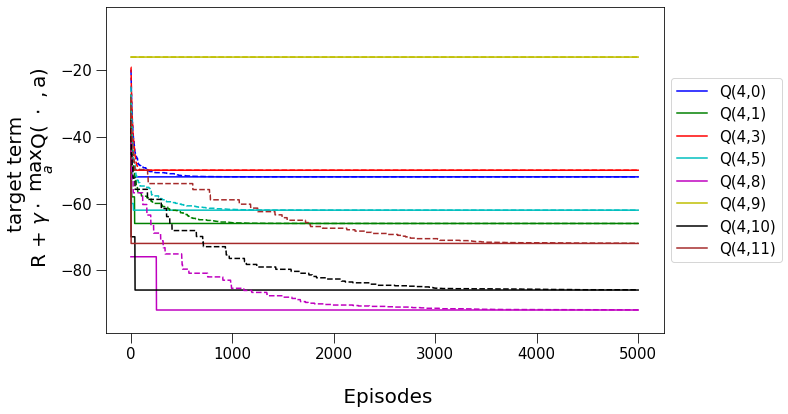
\includegraphics[width=0.9\textwidth]{figures/Reinforcement/targetQ4.png}
    \caption{Target term $R + \gamma \max_a Q(S', a)$ for all possible action in state 4 with $\alpha = 1.0$ (solid line), and $\alpha = 0.1$ (dashed line)}
    \label{fig:Q4 target}
\end{figure}

%\begin{table}[!htbp]
%\begin{adjustbox}{center}
%\begin{tabular}{@{\extracolsep{5pt}} ccccccc} 
%\\[-1.8ex]\hline 
%\hline \\[-1.8ex]
%& State & Action & Next State & Reward & Updated & Target Policy \\
%$t$ & $S_t$ & $A_t$ & $S_{t+1}$ & $R_{t+1}$ & $Q(S_t, A_t)$ & $\max_a Q(S_t, a)$\\ 
%\hline \\[-1.8ex] 
%0 & 6 & 2 & 2 & -11 & -4.16 & [2] \\
%1 & 2 & 1 & 1 & -21 & -4.20 & [0] \\
%2 & 1 & 2 & 2 & -21 & -4.20 & [4] \\
%3 & 2 & 0 & 0 & -21 & -4.17 & [7] \\
%4 & 0 & 4 & 4 & -18 & -3.42 & [5] \\
%5 & 4 & 10 & 10 & -35 & -3.50 & [11] \\
%6 & 10 & 4 & 4 & -35 & -3.50 & [4] \\
%7 & 4 & 10 & 10 & -35 & -7.00 & [11] \\
%8 & 10 & 4 & 4 & -35 & -6.65 & [4] \\
%9 & 4 & 11 & 11 & -28 & -2.80 & [9] \\
%10 & 11 & 4 & 4 & -28 & -2.96 & [4] \\
%11 & 4 & 9 & 9 & -16 & -3.04 & [0, 3] \\
%\hline \\[-1.8ex] 
%\end{tabular}
%\end{adjustbox}
%  \caption{Quadruple of events $(S_t, A_t, S_{t+1}, R_{t+1})$, updated $Q(S_t, A_t)$, and the target policy in the %second episode of the training}
%  \label{tab:the second episode} 
%\end{table}

%\begin{table}[!htbp]
%\small
%\begin{adjustbox}{center}
%\begin{tabular}{@{\extracolsep{5pt}} ccccccc} 
%\\[-1.8ex]\hline 
%\hline \\[-1.8ex]
%& State & Action & Next State & Reward & Updated & Target Policy \\
%$t$ & $S_t$ & $A_t$ & $S_{t+1}$ & $R_{t+1}$ & $Q(S_t, A_t)$ & $\max_a Q(S_t, a)$\\ 
%\hline \\[-1.8ex] 
%0 & 6 & 2 & 2 & -11 & -52.244 & [2] \\
%1 & 2 & 7 & 7 & -22 & -46.172 & [3] \\
%2 & 7 & 2 & 2 & -22 & -45.969 & [2] \\
%3 & 2 & 3 & 3 & -10 & -42.218 & [3] \\
%4 & 3 & 4 & 4 & -17 & -32.842 & [4] \\
%5 & 4 & 9 & 9 & -16 & -15.998 & [9] \\
%\hline \\[-1.8ex] 
%\end{tabular}
%\end{adjustbox}
%  \caption{Quadruple of events $(S_t, A_t, S_{t+1}, R_{t+1})$, updated $Q(S_t, A_t)$, and the target policy in the %88th episode of the training}
%  \label{tab:the 88th episode} 
%\end{table}
\clearpage






 










